% Chapter 4
\chapter{实验设计及其结果}
\section{实验准备}
为了成功完成哮喘检测实验,系统需要准备的工具有:Android应用程序(用来收集咳嗽音频,并存储在本地内存中)以及装有tensorflow和matlab环境的笔记本电脑(用来提取音频特征并进行对音频进行分类)

在实验数据采集阶段,本人联系了武汉市中南医院呼吸科找到了4名患有哮喘的病人分别采集了10min左右的咳嗽信号,并利用咳嗽检测网络筛选了300组有效的单周期咳嗽信号,作为本系统的正样本数据。紧接着本人联系了5名身体健康的志愿者共收集了500组负咳嗽样本数据。
\section{咳嗽检测网络测试}
对应已经收集到的咳嗽信号,系统要对咳嗽事件进行正确的检测,去除样本中噪音大或者非咳嗽的样本,因此系统需要训练一个鲁棒性良好的咳嗽检测网络。

本网络的数据是使用Kvapilova L等人\cite{kvapilova2019continuous}的采集咳嗽样本作为正样本进行训练,将咳嗽样本与一些背景噪声混合以使其更加真实,从而达到扩大数据集的目的,背景噪音来自于musan数据集\cite{musan2015},其中噪音比为0.15。最终系统利用在数据采集阶段收集到的咳嗽样本(包括正常人咳嗽样本和病人咳嗽样本)对真实的样本进行分类检测。来观察训练出的网络对真实样本分类的有效性。
\subsection{参数重要性分析}
系统利用初步网络训练对参数的重要性和相关度进行分类。
\begin{table}[h]
\centering
\begin{tabular}[width=0.6\textwidth]{ccc}
\hline
\textbf{参数}                           & \textbf{重要性}                                     & \textbf{相关度}                                      \\ \hline
{\color[HTML]{343434} \textbf{drop1}} & {\color[HTML]{6434FC} \textbf{0.041}}            & {\color[HTML]{009901} \textbf{0.243}}             \\
\textbf{conv3}                        & {\color[HTML]{6434FC} \textbf{0.063}}            & {\color[HTML]{009901} \textbf{0.133}}             \\
conv2                                 & {\color[HTML]{6434FC} 0.071}                     & {\color[HTML]{009901} 0.124}                      \\
\textbf{drop2}                        & {\color[HTML]{6434FC} \textbf{0.038}}            & {\color[HTML]{009901} \textbf{0.091}}             \\
\textbf{conv4}                        & {\color[HTML]{6434FC} \textbf{0.047}}            & {\color[HTML]{009901} \textbf{0.089}}             \\
batch\_size                           & {\color[HTML]{6434FC} 0.041}                     & {\color[HTML]{009901} 0.041}                      \\
lr                                    & \multicolumn{1}{l}{{\color[HTML]{6434FC} 0.048}} & \multicolumn{1}{l}{{\color[HTML]{009901} 0.028}}  \\
conv1                                 & \multicolumn{1}{l}{{\color[HTML]{6434FC} 0.050}} & \multicolumn{1}{l}{{\color[HTML]{FE0000} -0.021}} \\
pool1                                 & \multicolumn{1}{l}{{\color[HTML]{6434FC} 0.432}} & \multicolumn{1}{l}{{\color[HTML]{FE0000} -0.113}} \\
beta2                                 & \multicolumn{1}{l}{{\color[HTML]{6434FC} 0.013}} & \multicolumn{1}{l}{{\color[HTML]{FE0000} -0.121}} \\
alpha                                 & \multicolumn{1}{l}{{\color[HTML]{6434FC} 0.050}} & \multicolumn{1}{l}{{\color[HTML]{FE0000} -0.257}} \\
beta1                                 & \multicolumn{1}{l}{{\color[HTML]{6434FC} 0.106}} & \multicolumn{1}{l}{{\color[HTML]{FE0000} -0.274}} \\ \hline
\end{tabular}
\caption{模型参数重要性分析}
\end{table}

该表显示了不同的超参数对“真实样本准确率”的影响。第一列显示了参数的重要性,第二列显示了与参数更改量之间的相关性,以及参数增加是否改善或恶化了参数。通过准确性得分,系统可以看到\(\beta_1\)、\(\beta_2\)以及\(\alpha\)对系统的影响很小,因为没有任何变化带来了性能提升。但同时几个卷积层以及损失函数对本网络的数据影响很大,但尚未经过足够的测试,应对此进行调查。
\subsection{模型参数调整}
本节为对于咳嗽检测网络进行网络模型训练的参数调整确认。通过调整系统的参数,实验验证了不同的系统参数对于模型的影响。

由上节的分析系统可以看出参数中卷积层的大小以及损失函数对模型的效果影响最大。所以需要选取适宜的网络的损失函数和子图数目。通过初步筛选,系统将损失函数确定为:交叉熵损失函数和最大似然损失函数两种。假定训练时所有条件均保持不变,按照第三章的网络结构进行设计,即在卷积核大小为\(5\times5\),池化核大小为\(2\times2\),训练集为1800,batch数目为128,训练次数为50,优化器采用Adam的条件下进行训练对比,其结果如下:
\begin{table}[h]
\centering
\begin{tabular}{cccc}
\hline
\textbf{损失函数/子图数}                                 & \textbf{验证集准确率}                        & \textbf{训练集准确率}                        & \textbf{真实样本准确率}                       \\ \hline
{\color[HTML]{FE0000} \textbf{交叉熵/(16,16,32,32)}} & {\color[HTML]{FE0000} \textbf{0.9756}} & {\color[HTML]{FE0000} \textbf{0.9673}} & {\color[HTML]{FE0000} \textbf{0.8941}} \\
交叉熵/16,16,16,32                                   & 0.9732                                 & 0.9682                                 & 0.8888                                 \\
最大似然/16,16,32,32                                  & 0.9672                                 & 0.969                                  & 0.8574                                 \\
交叉熵/32,32,32,32                                   & 0.9731                                 & 0.9663                                 & 0.862                                  \\
最大似然/16,16,16,32                                  & 0.9142                                 & 0.9008                                 & 0.708                                  \\
最大似然/32,32,32,32                                  & 0.9678                                 & 0.9669                                 & 0.8914                                 \\ \hline
\end{tabular}
\caption{调整损失函数和子图数对模型的影响}
\end{table}

通过表格系统可以看到当系统使用交叉熵函数作为系统的损失函数且子图数选取为16,16,32,32时样本分类准确性和真实数据分类准确率最高,到达了89.4\%基本适用于进行咳嗽的检测。
\subsection{模型决策修正}
在模型参数调整阶段,系统已经将真实样本的决策准确率提高到89\%。系统可以知道单周期的咳嗽音频信号可能难以特别准确分类(到达99\%)以上,所以说系统修改分类判断,对一段时间内多次的连续的咳嗽信号进行联合分类判断,用于修正模型的决策过程,具体理论以及决策过程如下:
\begin{enumerate}
    \item 存储连续N个连续的咳嗽音频信号,进行单周期的分类决策。
    \item 如果N个信号中,有T个信号及其以上的信号判断一致时,系统采取该判定值为本次连续分类决策的最终结果。
    \item 否则回到第一步,重新存储N个连续信号,进行联合分类决策
\end{enumerate}

在上述的理论情况下,系统使用公式\ref{eq:3.3}估算当N=3,T=2时联合分类决策的错误率:
\begin{equation}
    \label{eq:3.3}
    ErrorRate = C_4^3\times(0.11)^3\times0.89+0.11^4 \approx 0.488477\%
\end{equation}
以上理论表明,即使单周期咳嗽音信号的识别率在89\%左右,但是通过四次连续的联合分类决策,可以将识别率提升到99.5\%左右,系统按照此方法对网络进行训练以及预测,其网络结果如\ref{fig:xunlian-image}。最终的分类成功率在99\%左右。
    \begin{figure}[h]
      \centering
      \begin{subfigure}{0.4\textwidth}
        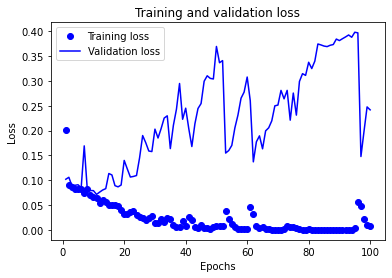
\includegraphics[width=\linewidth]{figures/100.png}
        \caption{训练阶段损失函数变化}
      \end{subfigure}
      \begin{subfigure}{0.4\textwidth}
        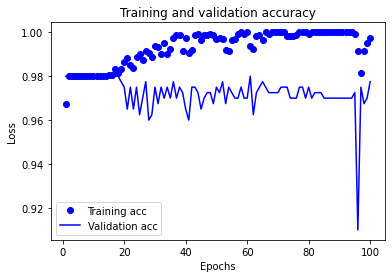
\includegraphics[width=\linewidth]{figures/100轮 准确性.png}
        \caption{训练阶段准确率变化}
      \end{subfigure}
      \caption{CNN训练过程展示}
      \label{fig:xunlian-image}
    \end{figure}
\section{支持向量机网络测试}

特征提取系统结构中论述所示,系统通过人工设计特征以及迁移学习获取了700多维度的特征向量并使用PCA降维最终形成长度为118的特征向量。如前所述,系统考虑了两种不同的支持向量机分类器,线性支持向量机和带RBF核的支持向量机(RBF-SVM)进行性能比较。在每一种情况下,训练和测试的准确性值被记录在大量(5000)的随机分区中,对于在10:90和90:10之间选择的各种训练测试的划分比,其平均值(标准差在括号中)列于表中。

\begin{table}[h]
\caption{样本相同,不同训练测试集划分比,不同SVM的分类结果}
\begin{tabular}{c|cc|cc}
\hline
                                     & \multicolumn{2}{c|}{\textbf{线性SVM}}                         & \multicolumn{2}{c}{\textbf{RBF-SVM}}                                          \\ \cline{2-5} 
\multirow{-2}{*}{\textbf{训练-测试集合比率}} & \textbf{训练集准确率}              & \textbf{测试集准确率}              & \textbf{训练集准确率}                       & \textbf{测试集准确率}                       \\ \hline
{\color[HTML]{343434} 10:90}         & {\color[HTML]{333333} 91.27} & {\color[HTML]{333333} 75.03} & {\color[HTML]{333333} 99.38}          & {\color[HTML]{333333} 78.97}          \\
20:80                                & {\color[HTML]{333333} 91.51} & {\color[HTML]{333333} 82.26} & {\color[HTML]{333333} 98.81}          & {\color[HTML]{333333} 84.32}          \\
30:70                                & {\color[HTML]{333333} 92.04} & {\color[HTML]{333333} 85.56} & {\color[HTML]{333333} 97.88}          & {\color[HTML]{333333} 86.66}          \\
40:60                                & {\color[HTML]{333333} 92.26} & {\color[HTML]{333333} 87.31} & {\color[HTML]{333333} 98.86}          & {\color[HTML]{333333} 88.11}          \\
50:50                                & {\color[HTML]{333333} 92.24} & {\color[HTML]{333333} 88.40} & {\color[HTML]{333333} 98.86}          & {\color[HTML]{333333} 88.89}          \\
60:40                                & {\color[HTML]{333333} 92.27} & {\color[HTML]{333333} 89.02} & {\color[HTML]{333333} 98.46}          & {\color[HTML]{333333} 89.58}          \\
70:30                                & {\color[HTML]{333333} 92.31} & {\color[HTML]{333333} 89.53} & {\color[HTML]{333333} 98.62}          & {\color[HTML]{333333} 90.10}          \\
80:20                                & {\color[HTML]{333333} 92.26} & {\color[HTML]{333333} 89.88} & {\color[HTML]{333333} 98.65}          & {\color[HTML]{333333} 90.55}          \\
90:10                                & {\color[HTML]{333333} 92.25} & {\color[HTML]{333333} 89.60} & {\color[HTML]{333333} \textbf{98.86}} & {\color[HTML]{333333} \textbf{90.83}} \\ \hline
\end{tabular}
\end{table}

显然,对于线性支持向量机,平均训练和测试准确率水平随着训练测试比的增加而增加,但也有少数例外。正如预期,随着训练数据的可用性的增加,该分类器往往学习得更好。对于RBF-SVM模型中,系统所得到的平均测试精度,仍然很大程度上遵循上述增加的趋势,比使用线性支持向量机获得的每个分裂比略有改善。这表明了潜在问题中固有的中等程度的非线性。尽管在测试精度上只有轻微的提高,但平均训练精度的提高明显更高,这表明RBF核在建模方面训练数据的某些非线性方面,而这些方面不能很好地一般化划分。

实际上,考虑标准差值也可以得出类似的结论如下。在线性SVM和BBF-SVM两种模型中训练精度的标准差都随着划分比的增加而减小,并且后者的值明显更低,表明RBF-SVM建模效果更好。然而,从测试精度来看,当划分比值较低时,RBF-SVM的标准差较低,当划分比值较高时,线性SVM的标准差较低。这一现象表明系统泛化性能较差。随着划分比的增加,两种情况下的标准差先减小后增大可以看出细微的差别。而测试的准确性是最可靠的(即,具有最低的标准偏差),在线性SVM的情况下(也在[26]其他地方观察到)一个均匀的划分训练测试比,在RBF-SVM的情况下,最高的可靠性是在划分比40:60观察到。
\begin{table}[h]
\centering

\begin{tabular}{cccc}
\hline
\multicolumn{1}{l}{{\color[HTML]{000000} }}      & {\color[HTML]{000000} \textbf{预测\textbackslash{}真实}} & {\color[HTML]{000000} \textbf{哮喘}} & {\color[HTML]{000000} \textbf{健康}} \\ \hline
{\color[HTML]{000000} }                          & {\color[HTML]{000000} 哮喘}                            & {\color[HTML]{000000} 89.47}       & {\color[HTML]{000000} 7.75}        \\
\multirow{-2}{*}{{\color[HTML]{000000} 线性SVM}}   & {\color[HTML]{000000} 健康}                            & {\color[HTML]{000000} 10.53}       & {\color[HTML]{000000} 92.25}       \\
{\color[HTML]{000000} }                          & {\color[HTML]{000000} 哮喘}                            & {\color[HTML]{000000} 91.61}       & {\color[HTML]{000000} 11.41}       \\
\multirow{-2}{*}{{\color[HTML]{000000} RBF-SVM}} & {\color[HTML]{000000} 健康}                            & {\color[HTML]{000000} 8.39}        & {\color[HTML]{000000} 88.59}       \\ \hline
\end{tabular}
\caption{训练测试集划分比为80:20的预测混淆矩阵(\%)}
\end{table}

虽然对于健康类,线性支持向量机在准确性和可靠性方面略优于RBF-SVM。请注意,给定疾病类别的RBF-SVM相对于线性SVM的优势与给定健康类别的线性SVM相对于RBF-SVM的优势是相似的。然而,由于给出患病类比给出健康类会产生更高的实际代价,因此应该选择RBF-SVM作为筛选工具。

综上考虑系统用80:20划分条件下,RBF-SVM的支持向量机。此时RBF-SVM对健康类的正确率为\textbf{88.59\%}对于哮喘类的正确率为\textbf{91.61\%},标准差分别为\textbf{7.09\%}和\textbf{8.82\%}。